\section{genericVcAllocator.h File Reference}
\label{genericVcAllocator_8h}\index{genericVcAllocator.h@{genericVcAllocator.h}}
{\tt \#include \char`\"{}../interfaces/networkComponent.h\char`\"{}}\par
{\tt \#include \char`\"{}../../../util/genericData.h\char`\"{}}\par
{\tt \#include $<$algorithm$>$}\par


Include dependency graph for genericVcAllocator.h:\nopagebreak
\begin{figure}[H]
\begin{center}
\leavevmode
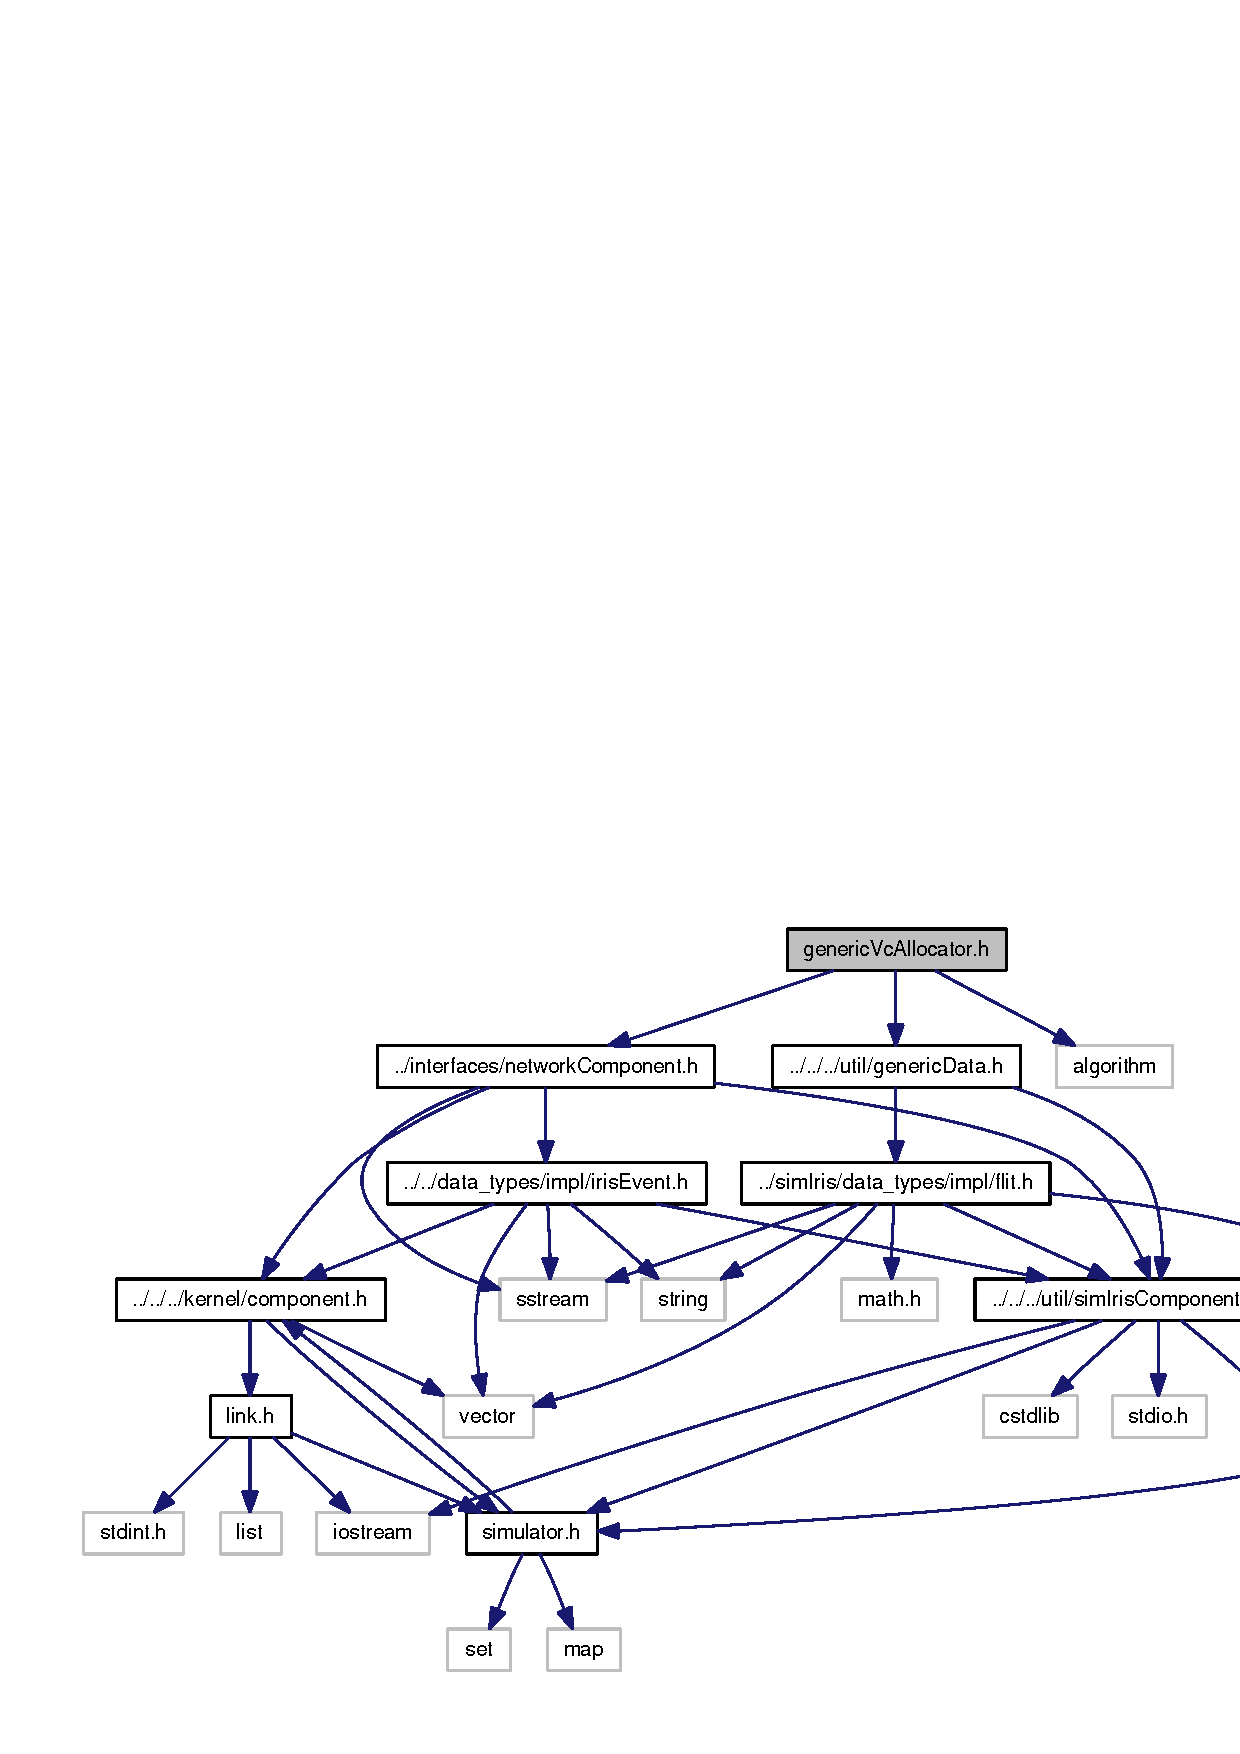
\includegraphics[width=339pt]{genericVcAllocator_8h__incl}
\end{center}
\end{figure}


This graph shows which files directly or indirectly include this file:\nopagebreak
\begin{figure}[H]
\begin{center}
\leavevmode
\includegraphics[width=279pt]{genericVcAllocator_8h__dep__incl}
\end{center}
\end{figure}
\subsection*{Classes}
\begin{CompactItemize}
\item 
struct {\bf VCA\_\-unit}
\item 
class {\bf GenericVcAllocator}
\begin{CompactList}\small\item\em This class allocates an output virtual channel to all requesting input messages. Only head flits pass through VCA. =====================================================================================. \item\end{CompactList}\end{CompactItemize}
\subsection*{Typedefs}
\begin{CompactItemize}
\item 
typedef struct {\bf VCA\_\-unit} {\bf VCA\_\-unit}
\end{CompactItemize}


\subsection{Typedef Documentation}
\index{genericVcAllocator.h@{genericVcAllocator.h}!VCA\_\-unit@{VCA\_\-unit}}
\index{VCA\_\-unit@{VCA\_\-unit}!genericVcAllocator.h@{genericVcAllocator.h}}
\subsubsection[{VCA\_\-unit}]{\setlength{\rightskip}{0pt plus 5cm}typedef struct {\bf VCA\_\-unit} {\bf VCA\_\-unit}}\label{genericVcAllocator_8h_7b7b7aa167e6c05a95a72e97478f1275}




Definition at line 34 of file genericVcAllocator.h.